%%%%%%%%%%%%%%%%%%%%%%%%%%%%%%%%%%%%%%%%%%%%%%%%%%%%%%%%%%%%%%%%%%%%%%%%%%%%%%%%%%%%%%%%%%%%%%%%%%%%%%
%
%   Filename    : chapter_1.tex 
%
%   Description : This file will contain your Research Description.
%                 
%%%%%%%%%%%%%%%%%%%%%%%%%%%%%%%%%%%%%%%%%%%%%%%%%%%%%%%%%%%%%%%%%%%%%%%%%%%%%%%%%%%%%%%%%%%%%%%%%%%%%%

\chapter{Research Description}
\label{sec:researchdesc}    %--note: labels help you with hyperlink editing (using your IDE)

\section{Background of the Study}
Games in the form of digital display, video games have been around nearly as old as the early development of the first computers. In October of 1958, Physicist  William Higinbotham created what is believed to be the very first video game, a very simple game of tennis but in the form of an electronic display, controlling the ‘rackets’ up-and-down with a knob to hit the bouncing ball on the screen. Higinbotham spent two weeks planning and creating the device for the game, and after some debugging, the very first video game debuted with the name Tennis for Two (American Physical Society, 2008). Video games are often made for the main purpose of entertainment as a form of recreational activity. However, by definition, a video game is the mode of interaction between a player, or a group of players, and a machine with the help of an electronic display, which follows a “meaningful fictional context,” and establishes an emotional attachment between the players and the results of their actions within the fictional context (Bergonse, 2017). Nowadays, there are a wide range of video games available. Ranging from different genres such as role-playing games (RPGs), first-person shooters (FPS) games, fighting games, and many others. \figref{fig:moderngames} shows some of the most popular games today including League of Legends, Dota 2, and Counter-Strike: Global Offensive.

%--- the following example shows how to include a figure in PNG format
\begin{figure}[h]                %-- use [t] to place figure at top, [b] to place at the bottom, [h] for here
   \centering                    %-- use this to center the figure
   
\includegraphics{moderngames.png}      %-- include image file named as "disneychart.png" 
   \caption{Some of the modern video games}
    \label{fig:moderngames}
\end{figure}


But other than for entertainment purposes, video games are also often used for different purposes such as educational and training applications. According to Mestadi (2018), serious games can be described as having the property of: a game, a mental contest, an interactive computer application, a digital game, a simulation, a virtual environment, a mixed reality/media. All of these being applied for different purposes in serious fields such as education, health, and government/corporate training. Serious games are the kind of video games that are made with the purpose of imparting specific beneficial effects to the users while using the fun elements of the game to keep the users engaged in the activity. Some aviation companies such as the Gleim Aviations offer flight training courses that utilize serious games such as their X-Plane flight training course, the training includes different pilot trainings for flight lessons, and also a flight simulation with the help of the ultra-realistic X-Plane flight simulator (Gleim Aviation, 2021). As shown in Figure 2, X-Plane flight simulator provides trainees a similar experience of flying an actual airplane with the help of excellent graphics, great flight models, and different sorts of realistic scenarios replicated in the simulation.

\begin{figure}[h]
   \centering                    
   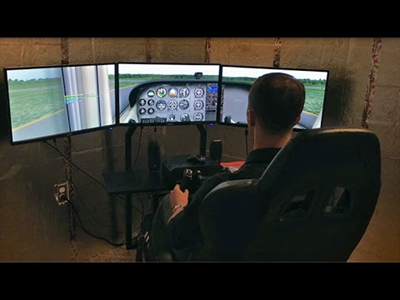
\includegraphics{flighttraining.png}
   \caption{Gleim X-Plane Flight Training Course Demonstration}
    \label{fig:flighttraining}
\end{figure}

Meanwhile, the application of serious games in the field of education has already been explored. This development did not come as a surprise since the purpose of developing serious games is to be used for educational purposes rather than entertainment. According to a meta-analysis conducted by Yu Zhongen (2018), one of the reasons why serious games are effective as a tool for education is because of its impact on the learners’ mood towards learning as an activity in this form of a game. An example of this educational serious game is Treefrog Treasure (n.d.), as shown in Figure 3. This is a type of platformer game developed for kids in the level of primary or elementary education. The goal of this game is to teach kids the concept of whole numbers, fractions, and percentages.

\begin{figure}[h]
   \centering                    
   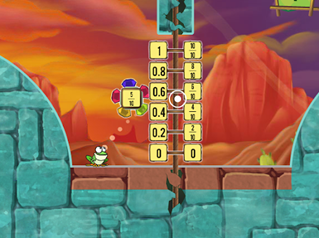
\includegraphics{treefrogtreasure.png}
   \caption{Treefrog Treasure}
    \label{fig:treefrogtreasure}
\end{figure}

When it comes to what makes a good serious game for teaching, Shute and Ke (2012) have synthesized their findings and derived seven core components of a well-designed serious game. Some of the derived components include:  Interactive problem solving, Specific goals/rules, adaptive challenges, ongoing feedback, and sensory stimuli. It is with these components that make a serious game provide an environment that promotes learning. In the study by Hassen Ben Rebbah (2019), they have shown that serious games have the potential to provide and/or promote intrinsic motivation of learners, situated learning, and learning from mistakes.

In global assessments for mathematics achievement, the Philippines has consistently ranked as one of the lowest in comparison to other countries. In 2018, the Philippines participated in the Programme for International Student Assessment (PISA) of the Organization for Economic Co-operation and Development (OECD), a triennial international assessment administered to 15-year old  learners, who are near the end of their compulsory basic education (Department of Health, n.d.). Released on the 3rd of December 2018, the PISA results revealed that Filipino students achieved an average score of 353 in Mathematical Literacy, which was significantly lower than the OECD average of 489 points. In addition to this, only 19.7 percent of Filipino students attained at least the minimum proficiency level in Mathematical Literacy.

Precalculus, a mathematics subject offered in Senior High School (SHS), is perceived to be difficult due to its concepts relying on formal definitions and proofs. In 2019, a study was conducted by Jaudinez in order to explore the teaching of SHS mathematics in the Philippines, and the results revealed that there were a number of problems when teaching precalculus to students. The identified problems include: lack of teaching strategies for difficult topics, lack of instructional resources, and lack of performance-based activities. Difficult topics were not abundantly reinforced, which caused teaching to be heavily dependent on the traditional way. Furthermore, lessons lack performance-based activities and tasks, and only conclude with practice exercises and tests. All the problems listed prior are factors to the low performance of students in procedural knowledge, computational skills, visualization, problem solving and other skills and processes in mathematics.

In order to design and develop a GBLE to target specific LOs in an educational game development, an Outcomes-Based Methodology could be followed (Sison et al, 2018). As Figure 4 shows, the first step in the GBLE development would involve identification of the LOs, followed by determining the genre of the game to be developed. After these two steps, the writing of the premise of the game would then be prioritized. This premise should clearly answer these three questions: (1) what is the player’s goal?, (2) how will the player achieve that goal?, and (3) what is the environment or world where the players will achieve the said goal? After this step, the next one would include designing the LO mechanics to be used as a game mechanic that would help the player-learners. This step is divided into achieving an LO, and then determining whether or not the LO has been achieved, and to what extent. This step involving the designing of the LO mechanics would repeat as long as it needs to take to completely build the GLE after the repeated designing and evaluation of the LO mechanics and related elements of it. The loop in the incremental development of the GLE might sometimes include a redesign for an LO mechanic based on its performance evaluation on the playtesting. Following this part of the methodology would include the integration of all the elements before proceeding to the final playtest and evaluation of the GBLE.

\begin{figure}[h]
   \centering                    
   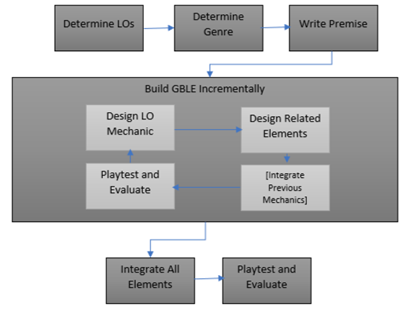
\includegraphics{outcomebased.png}
   \caption{Outcome-Based Methodology for Game-Based Learning Environment Development}
    \label{fig:outcomebased}
\end{figure}

The Philippines has constantly been placed among the lowest ranks in multiple indices regarding mathematics achievement. In the PISA 2018, students scored significantly lower than the OECD average, and in the Trends in International Mathematics and Science Study 2019 (TIMSS), the Philippines scored the lowest among all 58 participating countries (Magsambol, 2020). According to Jaudinez (2019), there were several problems when precalculus was being taught to students as revealed in his study in exploring the teaching of SHS Mathematics in the Philippines. One of the problems that were identified is the lack of teaching strategies for difficult topics. Teaching is heavily dependent on the traditional face to face method, and difficult topics were not reinforced causing students to have difficulty in learning and lose interest in the subject. In addition to this, although the Philippines has already adapted the outcomes-based education approach in schools, the outcomes-based methodology still has not been applied to the design and development of a SHS precalculus GBLE.

\section{Research Objectives}
\label{sec:researchobjectives}

In this section, we define the research objectives that guide this thesis. These objectives serve to focus the study, providing clear goals that aim to address the research questions posed. This thesis aims to achieve the following objectives:

\begin{subs}
\subsection{General Objective}
\label{sec:generalobjective}

To design, develop, and evaluate a Game-Based Learning Environment (GBLE) that supports in teaching Senior High School (SHS) Precalculus pedagogy. The GBLE will be evaluated for its ability to support the achievement of select learning outcomes of the said subject, as well as for its ability to engage player-learners.

\subsection{Specific Objectives}
\label{sec:specificobjectives}

The specific objectives for this study are as follows:

\begin{enumerate}
   \item To review challenges in Senior High School (SHS) Precalculus pedagogy;
   \item To identify target learning outcomes (LO) from SHS Precalculus;
   \item To design LO mechanics that support the achievement of the target LOs identified;
   \item To develop a Game-Based Learning Environment (GBLE) incorporating the LO mechanics identified; and
   \item To determine the effects of the GBLE in terms of supporting the achievement of the target LOs and the engagement of player-learners
\end{enumerate}
\end{subs}

\section{Scope and Limitations of the Research}
\label{sec:scopelimitations}

The goal of the study is to design, develop and evaluate a game-based learning environment (GBLE) that  would support senior high school precalculus pedagogy. The GBLE to be developed is intended to support the achievement of selected precalculus Learning Outcomes (LOs). Thus, player-learners are to play the GBLE while they are taking the topics covered by the selected LOs. It is not meant to introduce topics, nor is it meant to serve as an assessment tool for SHS Precalculus.

\begin{subs}
\subsection{Challenges in Senior High School Precalculus Pedagogy}
In order to identify challenges in SHS Precalculus Pedagogy, a literature review would be conducted. This literature review would include data from the Philippines as well as its neighboring countries in South East Asia (SEA). It is hoped that other Southeast Asian countries may have similar educational contexts as in the Philippines, and may have similar challenges. In the absence of enough data to identify pedagogical challenges, the literature review would be expanded to include other countries outside SEA that may have the same educational contexts as the Philippines.

\subsection{Learning Outcomes of Precalculus}
In order to identify target LOs from SHS Precalculus, the 2019 SHS Curriculum Guide (SHS-CG) from the Department of Education (DepEd) would be reviewed. In addition, a SHS Precalculus context expert would be consulted. Identifying LOs will be time consuming because the process should be as thorough as possible for there are things to be considered. In choosing LOs, the difficulty of the topics in the curriculum, the need of assistance from a third party for certain topics, and how applicable the development of GBLE will be for the LOs should all be considered first before deciding which LOs should be used. The LOs that translate the best into a GBLE, as decided upon by consultations with the context expert would be selected. Following the Outcomes-Based Methodology of Sison et al (2018), once target LOs have been identified, LO mechanics that target the LOs would be designed.

Based on the advice of the research adviser and the context expert, the chosen target LOs were chosen from the Department of Education’s curriculum guide for Senior High School STEM Course (2019). The target LOs were from the Analytical Geometry content which mainly discusses Conic Sections. The target LOs were: Learning Competency No. 14: to recognize the equation and important characteristics of the different type of conic sections, and Learning Competency No. 15: to solve situational problems involving conic sections.

\subsection{Learning Outcomes Mechanics}
In order to adhere to the aforementioned methodology, and to rapidly develop the GBLE, these LO mechanics would be integrated, playtested and evaluated periodically by the proponents of the study along with the context expert and research adviser. These LO mechanics would be part of the core gameplay loop of the GBLE. To support the LO mechanics, several non-LO mechanics may be designed, but they would not be prioritized for the study and would only be designed to support the core gameplay loop of the GBLE. The GBLE to be developed will be for desktop computers, which can run more powerful software compared to other devices such as consoles and mobile devices. Due to the transition from face-to-face classes to online classes, it is more likely that the participants will be able to undergo the experiment.

\subsection{Game-Based Learning Environment Design}
Developing the game would involve choosing a platform in which is the most available one for the player-learners. This is in consideration of the students that are at risk or vulnerable situations. Unity, a cross-platform game engine, would be used to develop the game because it has several features such as rendering, scripting, physics, and asset tracking that help reduce the time and cost for developing games. It also supports several platforms, allowing it to be easily shared between web, PC, and mobile platforms. 

Lastly, in order to determine the effect of the GBLE on the engagement and academic performance of the player-learners, a quasi-experiment would be done which involves assessing the difference in academic performance before and after the playtesting by comparing pre-test and post-test results. Only a quasi experiment will be used instead of true experimental research as there is only a limited time to gather data. Measures of statistical significance would be used in the comparison; should the desired number of n participants may be gathered, parametric tests would be used otherwise, non-parametric tests would have to be utilized.
\end{subs}

\section{Significance of the Research}
\label{sec:significance}

This study aims to develop a GBLE that would increase the engagement and academic performance of senior high school students and player-learners. Additionally, this study also aims to give instructors a new platform for teaching their students. The following individuals will benefit from this research: 

\begin{subs}
\subsection{Students}
This study can give students an alternative way of learning through the use of educational serious games. The game-based learning environment developed can be used by students as a support tool in their precalculus topics in order to further improve their knowledge and increase their motivation.

\subsection{Instructors}
This study can give instructors an alternative teaching method rather than the traditional face to face way, and the GBLE developed can be used by instructors as a support tool in teaching precalculus to their students in order to keep them more engaged in learning.

\subsection{Game Developers}
The GBLE developed can give game developers new ideas in designing and developing educational serious games, most especially in the domain of mathematics. Furthermore, game developers will be able to adapt the idea of what to prioritize first when creating games, such as focusing on the learning outcomes first before the design of the game itself.

\subsection{Future Researchers}
This study can assist future researchers given the knowledge of the processes involved when developing a GBLE. Furthermore, they will be able to use this paper as a reference for more studies related to this topic in the future.
\end{subs}

\section{Research Methodology}
The following are the sets of activities that will be performed in order to accomplish the objectives of the study:

\begin{figure}[h]
   \centering                    
   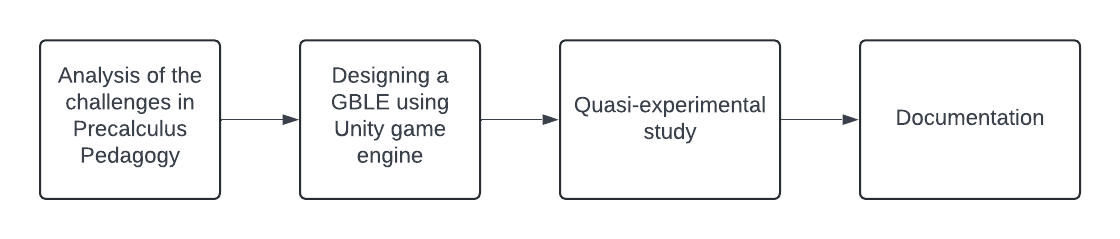
\includegraphics[scale=0.9]{studyflowchart.png}
   \caption{Step-by-step flowchart for the study}
    \label{fig:studyflowchart}
\end{figure}

\begin{figure}[h]
   \centering                    
   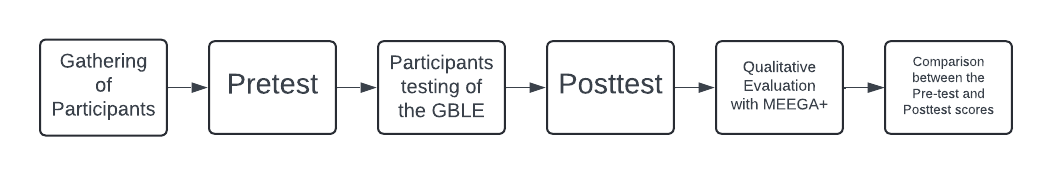
\includegraphics{quasiexperiment.png}
   \caption{Step-by-step flowchart for the Quasi-experiment}
    \label{fig:quasiexperiment}
\end{figure}

\begin{subs}
\subsection{Investigation of Precalculus Pedagogy}
Challenges in the practice of teaching Precalculus in senior high school students will be investigated. Various related works and literature will be reviewed and examined in relation to these challenges. The curriculum of SHS students for Precalculus will be observed in order to generate ideas regarding where the assistance of using GBLE would be most relevant. In addition to checking the curriculum, a SHS Precalculus professor will be consulted in order to find out the learning outcomes that students struggle with.

\subsection{Design of the GBLE}
An educational game would then be designed and developed using the Unity game engine to assist the students in learning precalculus. The game design and learning outcomes involved would be based on the gathered data and feedback from Precalculus professors and serious game developers. Before the designing of the game, the learning outcomes should first be designed in order to assess the features that will be in the game. This way, the content of the game will be centered around the important points of the LOs.

\subsection{Quasi-experimental Study}
The first process in the quasi-experiment with a one-group pretest-posttest design will be the gathering of the participants. The participants will take a pre-test assessment in order to evaluate their performance in Precalculus, and then undergo a 1 hour playtest or until game completion. The participants will then take a post-test assessment regarding their performance in Precalculus, and a survey will be conducted to measure their engageability and overall experience. When all the data has been collected, the data will be compared and will undergo statistical analysis through a paired t-test in order to determine if there is a significant difference in the pre-test and post-test scores.
Since the participants involved are all senior high school students which are mostly in the age range of 16-18 years old, appropriate consent forms would be provided for the student and their guardians. Names of the participating students would be kept confidential. All personal data that will be collected will be disposed of after being used in this study.
For the qualitative evaluation, a MEEGA+ questionnaire (2018) will be given to those students that tested the game to evaluate their feedback about their experience with the game. The test scores of two groups, and the MEEGA+ results from the game testers would be used to create a statistical analysis about the performance of the proposed GBLE.
\subsection{Documentation}
All the plans, evaluations, and implementations that were involved in this study such as the data collected and the different processes in creating a GBLE will be documented and maintained up-to-date within the duration of this study.
\subsection{Calendar of Activities}
The following tables shows the Gantt chart of the activities for 2021 and 2023:

Table \ref{tab:timetableactivities2021} and Table \ref{tab:timetableactivities2023} shows a Gantt chart of the activities.  Each bullet represents approximately one week worth of activity.

%
%  the following commands will be used for filling up the bullets in the Gantt chart
%
\newcommand{\weekone}{\textbullet}
\newcommand{\weektwo}{\textbullet \textbullet}
\newcommand{\weekthree}{\textbullet \textbullet \textbullet}
\newcommand{\weekfour}{\textbullet \textbullet \textbullet \textbullet}

%
%  alternative to bullet is a star 
%
\begin{comment}
   \newcommand{\weekone}{$\star$}
   \newcommand{\weektwo}{$\star \star$}
   \newcommand{\weekthree}{$\star \star \star$}
   \newcommand{\weekfour}{$\star \star \star \star$ }
\end{comment}

\begin{table}[h]   %t means place on top, replace with b if you want to place at the bottom
\centering
\caption{Timetable of Activities (2021)} \vspace{0.25em}
\begin{tabular}{|p{2in}|c|c|c|c|c|c|c|c|} \hline
\centering Activities (2021)            & Mar   & Apr & May & Jun & Jul & Aug & Sep \\ \hline
Review Serious Games \& Related Works   & \weekfour & \weekfour & \weekfour &  &  &  &  \\ \hline
Data Gathering for Senior High School Teaching Pedagogy    &   &  &  & \weekfour & \weekfour & \weekfour &  \\ \hline
GBLE Design      &   &  &  &  &  & \weekfour & \weekfour \\ \hline
Documentation & \weekfour  & \weekfour & \weekfour & \weekfour & \weekfour & \weekfour & \weekfour \\ \hline
\end{tabular}
\label{tab:timetableactivities2021}
\end{table}
\begin{table}[h]   %t means place on top, replace with b if you want to place at the bottom
\centering
\caption{Timetable of Activities (2024)} \vspace{0.25em}
\begin{tabular}{|p{2in}|c|c|c|c|c|c|c|} \hline
\centering Activities (2024)            & Feb & Mar & Apr & May & Jun & Jul \\ \hline
GBLE Development    & \weekfour & \weekfour & \weekfour & \weekfour & \weekfour &  \\ \hline
GBLE Testing        &   &   &   & ~~\weektwo  & \weekfour & \weekone~~~ \\ \hline
Data Collection     &   &   &   &   &   & \weektwo~~ \\ \hline
Results and Analysis&   &   &   &   &   & ~\weekone~~ \\ \hline
Documentation &  \weekfour & \weekfour & \weekfour & \weekfour & \weekfour & \weektwo~~~ \\ \hline
\end{tabular}
\label{tab:timetableactivities2023}
\end{table}

\end{subs}